% !TeX root = dissertation.tex
\chapter{Evaluate the Household IoT Privacy-setting Profiles and User Interfaces}\label{chapter:evaluation}

\section{Introduction}

In the previous chapters, we have described the three studies on recommending privacy settings for general/public IoT, household IoT, and fitness IoT, respectively. A ``data-driven” approach has been used in all three studies, to gain the underlying insights of IoT users' privacy decision behavior, and to design a set of User interfaces (UI) to incorporate the ``smart" privacy default/profiles created based on the insights. Users can apply these smart defaults/profiles by either a single click or by answering a few related questions. When applying this approach on the household IoT dataset in Chapter~\ref{chapter:householdIoT}, we explored the trade-off between parsimony and accuracy when creating the ``smart" privacy defaults/profiles. We manipulate the pruning parameter for the decision trees of the C4.5 algorithm, which impacted the complexity of the generated profiles based on the decision trees. Accuracy is important to ensure that users' privacy preferences are accurately captured and/or need only few manual adjustments, while parsimony, on the other hand, prevents overfitting and promotes fairness. In Chapter~\ref{chapter:householdIoT}, we noticed that more complex models tended to increase overall accuracy by predicting a few users' preferences more accurately, with no effect on other users. Parsimony also makes the associated default setting easier to understand for the user. 

The biggest limitation of our work so far is that we did not test any of the proposed UIs, so we do not know what level of complexity (both in terms of the user interface and the in terms of the profiles) is most suitable. Thus, to further test this trade-off between accuracy and parsimony in a real usage environment and test the user experience of using the interfaces that we designed in Chapter~\ref{chapter:householdIoT}, in this chapter, I address this limitation by discussing our final study on evaluating the new interface prototypes of recommending privacy-settings for household IoT. The main purpose of this study is to test the user experience of the privacy-setting profiles interfaces and defaults/profiles.


\section{Study Design}
In this chapter, we present the design our study, including the dependent variables and manipulations.
\subsection{Dependent Variables}
To test the user experience of our privacy-setting interfaces, the Dependent Variable of our study will be their \textbf{satisfaction to the system}, \textbf{and the trust to the company}, and several subjective system aspects, including \textbf{perceived usefulness}, \textbf{perceived ease of use}, \textbf{perceived privacy threats}, \textbf{perceived control}, \textbf{perceived privacy helpfulness}. As shown in Table~\ref{tab:cfa}, all the scales of these dependent variable are adapted from previous work.

\subsection{Manipulations}

\subsubsection{Interface complexity}
In Chapter~\ref{chapter:householdIoT},  we first designed a set of interfaces, as shown in Figure~\ref{fig:interface2}, based on the results from our statistical analysis (\textbf{UI1}). Further, we modified these interfaces to integrate the ``smart defaults/profiles" generated from our machine learning results. This modification separated the Storage and sharing modules from the Data usage, leading a slightly more complex interface design (\textbf{UI2}). For our study, we need to test these two groups of interfaces (UI1 vs UI2) in terms of interface complexity. Compared to UI1, UI2 has more granularity when setting on different storage. In UI1, users can only configure all the privacy-settings to be the same for the three different types of storage (Local, Remote, and Third-party sharing), while they can configure those setting for each type of storage differently in UI2.

\subsubsection{Profile complexity}
In terms of the complexity of ``smart defaults/profiles", we consider 4 different experimental conditions as follows:
\begin{itemize}
	\item \textbf{Everything-On}: With all the data access and usage being turned on, this is considered as the open default settings. This profile also means nothing has been done for the users. They have to make every change for themselves.
	\item \textbf{Everything-Off}: With all the data access and usage being turned off, this is considered as the most conservative default settings. In our previous studies, this is also the profile that more than 50\% participants want to use.
	\item \textbf{Smart Default}: One single ``smart profile" will be provided to the users. This is considered as the experimental condition with intermediate complexity.
	\item \textbf{Smart Profiles}: Multiple ``smart profiles" will be provided to the users. This is considered as the most sophisticated settings with high complexity in ``smart profiles".
\end{itemize}

These different default/profile conditions map to users' ``preference fit", where smart profiles and smart defaults conditions have better ``preference fit" than the two baseline conditions. In addition, smart profiles condition have more preference options for users to choose than smart default. Thus, we expect smart profile to have the best fit/user satisfaction or other subject system aspects, followed by smart defaults and the two baseline conditions.

From above, we have 2 different levels of interface complexity, and 4 different levels of profile complexity.
Hence, $4$x$2=8$ total experimental conditions (i.e., user interfaces) will be presented to the participants. 

\subsubsection{Profile/Interface Selection}
\textbf{Everything-Off} and \textbf{Everything On} profiles can easily be implemented on both our designed interfaces (UI1 and UI2).

For \textbf{Smart Default} and \textbf{Smart Profiles} selection, note that, when applying our machine learning algorithms in Chapter~\ref{chapter:householdIoT}, we have manipulated the pruning parameter to create different ``smart defaults/profiles". This manipulation results in a set of smart profiles with different weight in accuracy and parsimony. The more the decision tree is pruned, the less complex the resulting ``smart" profile will be, leading lower accuracy and high parsimony, and vice versa. Since we can only choose one ``smart default/profile" to test the interface, this selection needs to be done carefully.

\textbf{Smart Default:} In section~\ref{subsection:onerule2}, we have applied a one-rule algorithm to our dataset. The resulting ``smart default" in shown in Figure~\ref{fig:oneR}. This is the simplest ``smart default" settings across all the different ``smart defaults" settings with lowest accuracy (61.39\%) but highest parsimony. In addition, this ``smart default" can be easily integrate into both the \textbf{UI1} and \textbf{UI2}. Thus, we choose this ``smart default" as the target interface for experimental conditions \textbf{UI1:Smart Default} and \textbf{UI2:Smart Default}.
%. In contrast, we created a ``smart default" setting with only 8 nodes shown in Figure~\ref{fig:smart_default_new} in section~\ref{subsection:overall2}. This ``smart default" has the very high parsimony and the close to highest accuracy of 63.32\% across all the ``smart default" settings. In addition, this ``smart default" can be easily integrate into the \textbf{UI2}, the simpler interfaces. Thus, we choose this ``smart default" as the target interface for experimental condition --- \textbf{UI2:Smart Default}.

\textbf{Smart Profiles:} For ``smart profiles" selection, we want this interface differ as much as possible comparing the ``smart default", so we search across all the ``smart profiles" with large number of clusters. In addition, the ``smart profiles" should be easily integrated into UI1 or UI2. Figure~\ref{fig:conglo_5_profile001} is considered for UI1 because it has 5 clusters with a high accuracy of 80.35\%. And it has no interaction between \textbf{Storage} and other parameters. This is suitable for our UI1 design, serving as the target interface profiles for experimental condition --- \textbf{UI1:Smart Profiles}. We have separated the Data Storage and Data Usage modules in UI2. Thus, we choose Figure~\ref{fig:fit_5_profile003} for UI2 because it has 5 clusters, a close to highest accuracy of 83.11\%. In addition, in the cluster 3, it has a 2-way interaction between \textbf{Storage} and \textbf{Purpose}; in cluster 4, it has a 2-way interaction between \textbf{Storage} and \textbf{Action}. It does not have an 3-way interaction between any of these parameters in any of its clusters. Thus, we choose this set of ``smart profiles" as the target interface profiles for experimental condition --- \textbf{UI2:Smart Profiles}. We implemented above 8 different sets of user interfaces using HTML, PHP, CSS, and SQL.

\subsection{Research Questions}
%
%\begin{figure}
%	\centering
%	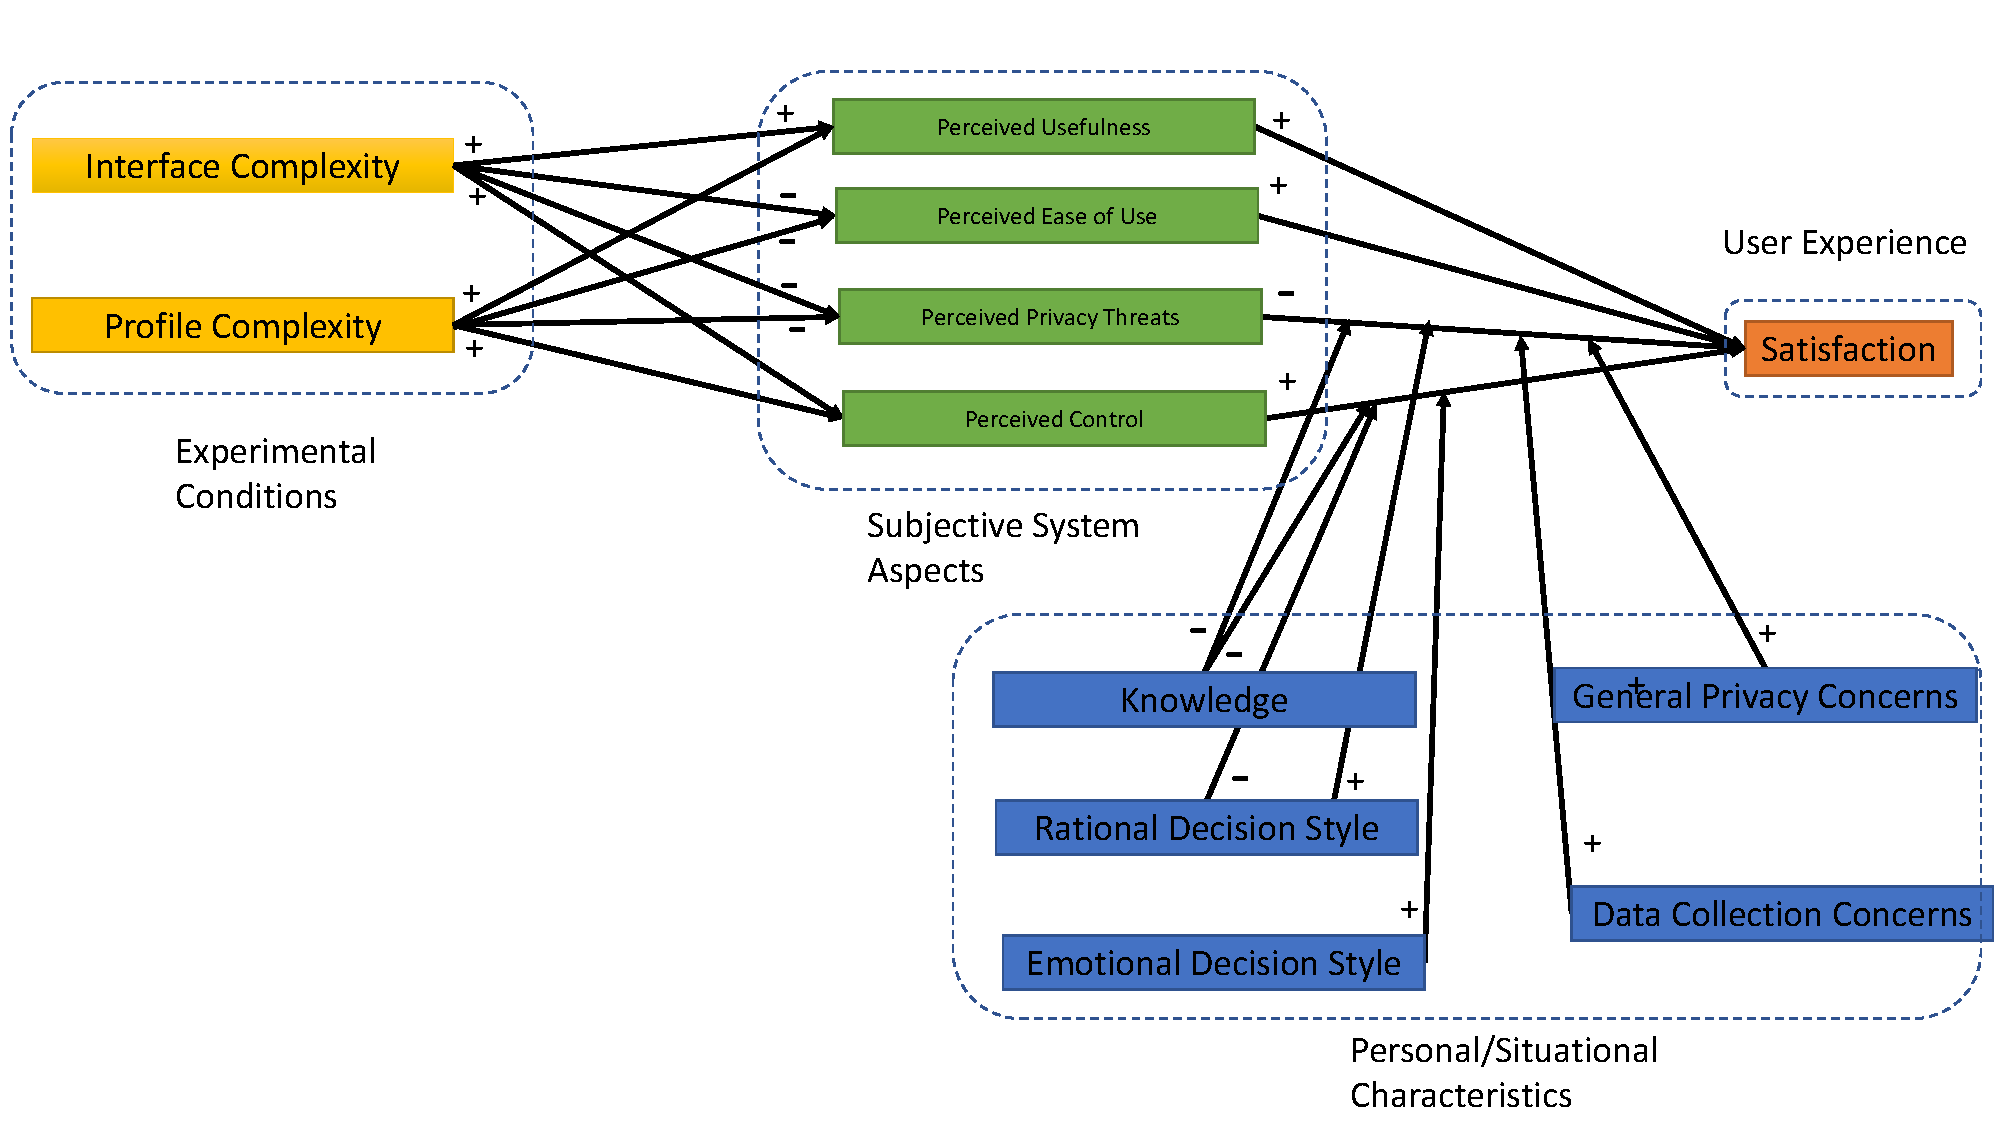
\includegraphics[width=\textwidth]{figures/uimodel.pdf}
%	\caption{Hypothesized effects on users’ experience and subjective evaluations.}
%	\label{fig:uimodel}
%\end{figure}

Compared to UI1, UI2 has more granularity when setting on different storage. In UI1, users can only configure all the privacy-settings to be the same for the three different types of storage (Local, Remote, and Third-party sharing), while they can configure those setting for each type of storage differently in UI2. Brandimarte et al. demonstrate that users perceive more control when privacy controls are more granular~\cite{brandimarte2013misplaced}. But this control can at times be an illusion. More granular controls allow users to set their privacy settings to a level that better reflects their privacy preferences, this additional control may increase the perceived usefulness~\cite{tang2012implications, al2016modeling}. Similarly, more fine-grained control may reduce users' perceived privacy threats. Tang et al. (2012) found that users of a finer-grained settings interface were more comfortable with their privacy settings. Research has also shown that increasing the control often introduces choice overload issues~\cite{iyengar2000choice, schwartz2004paradox, acquisti2005privacy, acquisti2007can}, which makes it more difficult and time-consuming for users to accurately their privacy settings~\cite{madejski2012study, sadeh2009understanding}.

Therefore, here are our first research question:
\theoremgroup
\begin{theorem}
	Is there any significant difference between UI1 and UI2 on users experience and other subjective system aspects when using our system?
\end{theorem}

%More granular controls allow users to set their privacy settings to a level that better reflects their privacy preferences, this addition control may increase the perceived usefulness~\cite{tang2012implications, al2016modeling}. Therefore, we hypothesize the following:
%\begin{theorem}
%	Users that use UI2 will perceived a higher usefulness compared to users that use UI1.
%\end{theorem}
%
%Similarly, more fine-grained control may reduce users' perceived privacy threats. Tang et al. (2012) found that users of a finer-grained settings interface were more comfortable with their privacy settings. Therefore, we hypothesize the following:
%\begin{theorem}
%	Users that use UI2 will perceived a lower privacy threats compared to users that use UI1.
%\end{theorem}
%
%Research has shown that increasing the control often introduces choice overload issues~\cite{iyengar2000choice, schwartz2004paradox, acquisti2005privacy, acquisti2007can}, which makes it more difficult and time-consuming for users to accurately their privacy settings~\cite{madejski2012study, sadeh2009understanding}. Therefore, we hypothesize the following:
%\begin{theorem}
%	Users that use UI2 will perceived a lower ease of use compared to users that use UI1.
%\end{theorem}

%\subsection{Profile Complexity and SSA}
In term of profile complexity, we have four different levels of experimental conditions. These different default/profile conditions map to users' ``preference fit". ``Smart profiles" provide the users more pre-configured options for users to choose from, leading to a better preference fit than the ``smart default" with only single ``smart" option provided, which in turn has a better fit than Everything-Off/Everything-On defaults. This additional freedom of choice and possible increased preference fit may increase the perceived control and perceived usefulness. Similarly, the increased preference fit may increase the level that the pre-configured profiles better reflect the users' privacy preferences, which may reduce the perceived privacy threats. The additional options in ``smart profiles" may introduce choice overload compared to the ``smart default" and Everything-Off and Everything-On defaults. This may lead to a low perceived ease of use for ``smart profiles". Compared to Everything-Off and Everything-On defaults, ``smart defaults" are generated from machine learning analysis results. The higher accuracy of ``smart defaults" can arguably result in fewer a lower manual changes that users would make to the system, leading to a higher perceived ease of use compared to Everything-Off and Everything-On defaults. Therefore, Here is our second research question:
\theoremgroup
\begin{theorem}
	Is there any significant difference between the 4 experimental conditions on users experience and other subjective system aspects when using our system?
\end{theorem}

%
%\theoremgroup
%\begin{theorem}
%	``smart profiles" interfaces will have the highest perceived control, followed by ``smart default". Everything-Off and Everything-On defaults will have the lowest perceived control.
%\end{theorem}
%\begin{theorem}
%	``smart profiles" interfaces will have the highest perceived usefulness, followed by ``smart default". Everything-Off and Everything-On defaults will have the lowest perceived usefulness.
%\end{theorem}
%
%Similarly, the increased preference fit may increase the level that the pre-configured profiles better reflect the users' privacy preferences, which may reduce the perceived privacy threats. Therefore, we hypothesize the following:
%\begin{theorem}
%	``smart profiles" interfaces will have the lowest perceived privacy threats, followed by ``smart default". Everything-Off and Everything-On defaults will have the highest perceived privacy threats.
%\end{theorem}
%
%The additional options in ``smart profiles" may introduce choice overload compared to the ``smart default" and Everything-Off and Everything-On defaults. This may lead to a low perceived ease of use for ``smart profiles". Compared to Everything-Off and Everything-On defaults, ``smart defaults" are generated from machine learning analysis results. The higher accuracy of ``smart defaults" can arguably result in fewer a lower manual changes that users would make to the system, leading to a higher perceived ease of use compared to Everything-Off and Everything-On defaults. Therefore, we hypothesize the following:
%\begin{theorem}
%	Controlling other conditions, ``smart default" interfaces will have the highest perceived ease of use, followed Everything-Off and Everything-On defaults. ``smart profiles" will have the lowest perceived ease of use.
%\end{theorem}

%\subsection{Personal/Situational Characteristics and SSA}
%Based on TAM and UTAUT that have been discussed in Chapter~\ref{chapter:Relatedwork1}, perceived usefulness can be increased by the benefits and advantages gained from the technology. In our study, perceived usefulness suggests the users will find the Household IoT privacy-setting interfaces that we designed are useful. Research has shown that perceived usefulness is a significant predictor of the intention to use IoT services~\cite{coughlan2012exploring}. Therefore, we hypothesize the following:
%\theoremgroup
%\begin{theorem}
%	Perceived usefulness will be positively associated with users' satisfaction with the system.
%\end{theorem}
%
%Similarly, the causal relationship between the perceived ease of use of setting interfaces and users' satisfaction with the system has been codsified in both TAM and UTAUT. Several research has also verified this causal relationship~\cite{gao2014unified, dong2017understanding, choi2016smartwatch}. Therefore, we hypothesize following:
%\theoremgroup
%\begin{theorem}
%	Perceived ease of use of the privacy-setting interfaces will be positively associated with users' satisfaction with the system.
%\end{theorem}
%
%Perceived privacy threats measure the level of privacy threatening regarding data collection of the users and control perceived by users when using the system. Higher perceived privacy threats will lead to a higher system-specific concern of privacy risks~\cite{knijnenburg2013persuasive, knijnenburg2014increasing}. Therefore, we hypothesize following:
%\theoremgroup
%\begin{theorem}
%	Perceived privacy threats will be negatively associated with users' satisfaction with the system.
%\end{theorem}
%
%The effect of perceived privacy threats on the system satisfaction may be moderated by the General Privacy Concerns and Data Collection Concerns. Research has shown that the negative association between over-sharing threat and system satisfaction will be stronger for users with a high level of Interpersonal privacy concerns~\cite{knijnenburg2014increasing}. However, for people with low Privacy  Concerns, the increased threat may not result in a reduced satisfaction with the system~\cite{hann2007overcoming, krasnova2009investigating}. Therefore, we hypothesize following:
%\begin{theorem}
%	The negative association between perceived threats and system satisfaction will be stronger for users with a high level of general privacy concerns or data collection concerns.
%\end{theorem}
%
%The positive effect of perceived control on the system satisfaction has been verified by a few research~\cite{malhotra2004internet, madejski2012study}. Therefore, we hypothesize following:
%\begin{theorem}
%	Perceived control will be positively associated with users' satisfaction with the system.
%\end{theorem}
%
%Knowledge measures how much the users know about the smart home devices. Users with a high level of knowledge may have a high level of expectations in data collection and control. When these users are evaluating the satisfaction with the system, the high level of expectation may moderate the effect of perceived privacy threats and perceived control. Therefore, we hypothesize following:
%\theoremgroup
%\begin{theorem}
%	The negative association between perceived threats and system satisfaction will be stronger for users with a high level of knowledge.
%\end{theorem}
%\begin{theorem}
%	The positive association between perceived control and system satisfaction will be weaker for users with a high level of knowledge.
%\end{theorem}

%The remaining hypotheses are related to the rational decision style and emotional decision style. To our knowledge, no research has been done in the IoT context regarding the effect of decision style on the effect of perceived privacy threats and perceived control. Even in our previous study discussed in Chapter~\ref{chapter:householdIoT}, we did not find a significant effect of rational or emotional decision style on the decision of contextual scenarios. We explored the effect of these personal characteristics in this chapter but no significant effects were found.

%Still, we make following hypothesis based on these thinking: 1) users with a high level of rational decision style make think more about concrete privacy risk, leading to more perceived privacy threats and less perceived control; 2) It may be easier for users with a high level of emotional decision style to think the system is complex, leading to a higher perceived control.
%\theoremgroup
%\begin{theorem}
%	The negative association between perceived threats and system satisfaction will be stronger for users with a high level of rational decision style.
%\end{theorem}
%\begin{theorem}
%	The positive association between perceived control and system satisfaction will be weaker for users with a high level of rational decision style.
%\end{theorem}
%\begin{theorem}
%	The positive association between perceived control and system satisfaction will be stronger for users with a high level of emotional decision style.
%\end{theorem}

\section{Experimental setup}

In this section, we discuss the Experimental setup of our user study. This user study will be a between-subject study, which takes about 15 -- 20 minutes to finish. All participants will be recruited via Amazon Mechanical Turk.

\subsection{Participants and Procedures}
Based on the power analysis results, to collect our dataset, 504 adult U.S.-based participants were recruited through Amazon Mechanical Turk. Participation was restricted to Mechanical Turk workers with a high reputation (at least 50 completed tasks, average accuracy of $> 96\%$). Participants were paid \$1.50 upon successful completion of the study. The participants were warned about not getting paid in case they failed attention checks (see below). The study participants represented a wide range of ages, with 44 aged 18-24, 298 aged 25-34, 116 aged 35-44, 29 aged 45-54, 12 aged 55-64, and 5 participants over 65 years old.

During the study~\footnote{The user study url can be found here: http://iot.usabart.nl/yang}, the participants were first welcomed with a brief introduction of the experimental instructions. We explicitly introduce that the goal of this study is to test a new setting interfaces for Smart Home Users.

Then each participant was shown a video with a brief introduction to various smart home devices, which also mentioned various ways in which the different appliances would cooperate and communicate within a home. After the video, participants were asked to answer two attention check questions depicted in Figure~\ref{fig:yangAttentionCheck} in the Appendix.

After the introduction video, each participant was shown the basics of our UI and usage instructions, shown in~Figure~\ref{fig:yangPrepage} in the Appendix. Then each participant was presented with one privacy-setting user interface for household IoT that was randomly choosen from the previous lydiscussed 8 different experimental conditions. Participants were asked to set all the privacy-settings to best fit their own privacy preferences. They were required to spend at least 25 seconds before they can leave the UI page and will be warned if they spent too little time on the UI page.

Finally, a post-test survey questionnaire was shown to each participant, asking their user experience using our privacy-setting interfaces. The questionnaire included three groups of questions -- \textit{experience} (i.e. satisfaction with the system); \textit{Subjective System Aspects} (SSA), including Perceived usefulness, Perceived ease of use, perceived privacy threats, perceived control); and \textit{personal/situational characteristics} (General privacy concerns, Data Collection Concerns, Knowledge, Rational Decision Style, and Emotional Decision Style). All items were adapted from previous published studies with minor modifications in wording to accommodate the IoT privacy-setting context. Each item was measured on five-point Likert scales with 1 being "strongly disagree" to 7 being "strongly agree". All the items of the questionnaire are shown in Appendix.

%After the user study is finished, We will first use \textit{confirmatory factor analysis} to clean up the items and then use \textit{linear mixed effects regression} to analyze the effect of the independent variables on the subjective system aspects, and further mediation effect on the user experience. We also wonder how the personal/situational characteristics affect the user experience.


\section{Results}
In this section, I present the statistical analysis results. I first discuss the confirmatory factor analysis that I conducted to clean up the survey question items. Then I discuss the structural equation model (SEM) that I used to analyze the effect of the independent variables on the subjective systems aspects and user experience. And finally, I present the effect of personal/situational characteristics on the subjective systems aspects and user experience.

\subsection{Confirmatory Factor Analysis}
I conducted a Confirmatory Factor Analysis (CFA) and examined the validity and reliability scores of the constructs measured in the study. I started with the saturated model, as shown in Figure~\ref{fig:cfasaturated}. Upon inspection of the CFA model, I removed items that have lowest R-square value since this means that this item explains the least percentage of the scale. 

During this process, th6 (low communality 0.121 ), e2 (low communality 0.221 ), e7 (low communality 0.237), th5 (low communality 0.222), s8 (low communality 0.233), th2 (low communality 0.278), u4 (low communality 0.291), e4 (low communality 0.330), e5 (low communality 0.341), e9 (low communality 0.311), tr2 (low communality 0.365), tr4 (low communality 0.353)
tr8 (low communality 0.209), tr3 (low communality 0.295), tr1 (low communality 0.246), s4 (low communality 0.317), s3 (low communality 0.274), s6 (low communality 0.298), e1 (low communality 0.308 ), e10 (low communality 0.184), u2 (low communality 0.368), u7 (low communality 0.346), s5 (low communality 0.383), s7 (low communality 0.327) were removed. Interestingly, after removing e10, I removed h4 (communality 0.612) instead of h2 (low communality 0.227), because if h2 was removed, both h1 and h3 need to be removed, leaving only one item in that scale. While if h4 was removed, h1, h2, and h3 can all be kept in the model.

And at the end, I also checked that no item has high cross-loadings with other factors. The remaining scale items with their R-square value of the trimmed model are shown in Table~\ref{tab:cfa}. The final trimmed model is shown in Figure~\ref{fig:cfafinalmodel}.

\begin{figure}
	\centering
	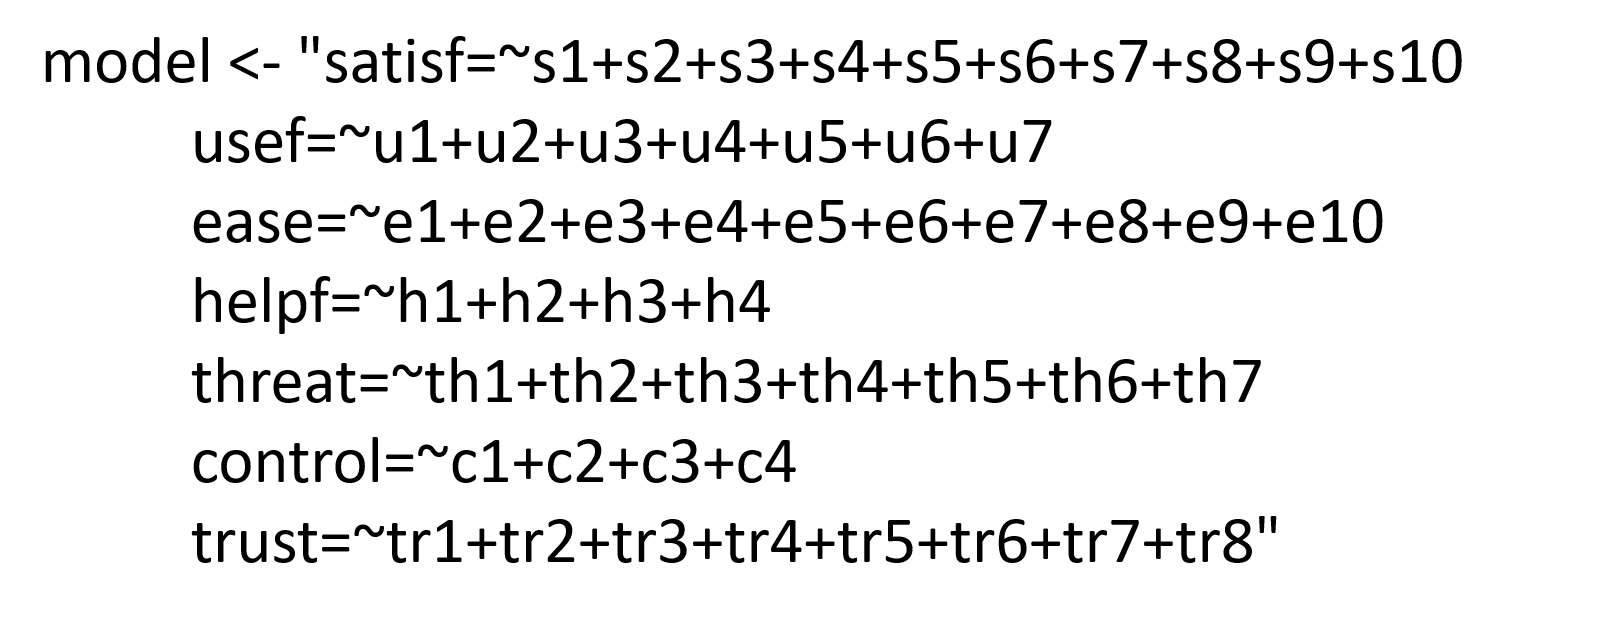
\includegraphics[width=0.7\textwidth]{figures/cfasaturated.png}
	\caption{CFA Saturated Model.}
	\label{fig:cfasaturated}
\end{figure}

%\begin{figure*}[t!]
%	\centering
%	\begin{subfigure}[t]{0.5\textwidth}
%		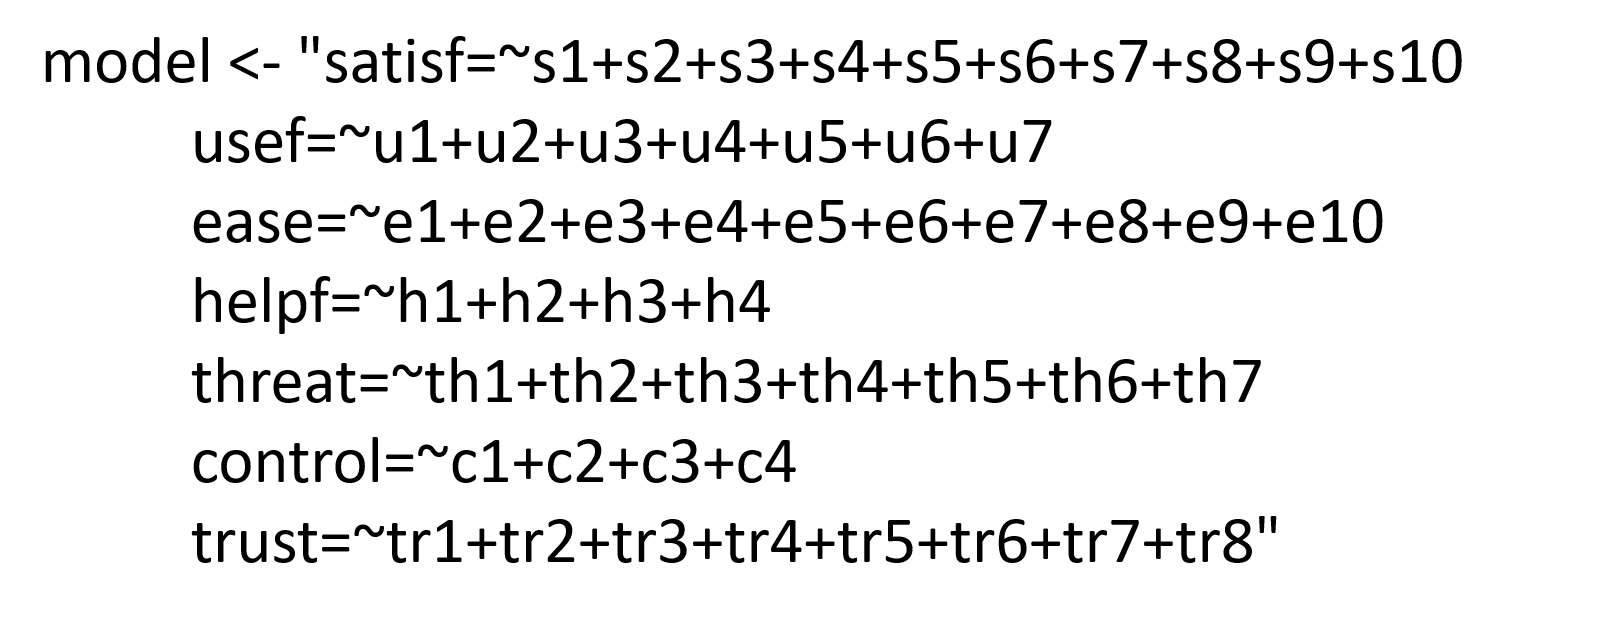
\includegraphics[t]{figures/cfasaturated.png}
%		\caption{CFA Saturated Model.}
%		\label{fig:cfasaturated}
%	\end{subfigure}%
%	~ 
%	\begin{subfigure}[t]{0.5\textwidth}
%		\centering
%		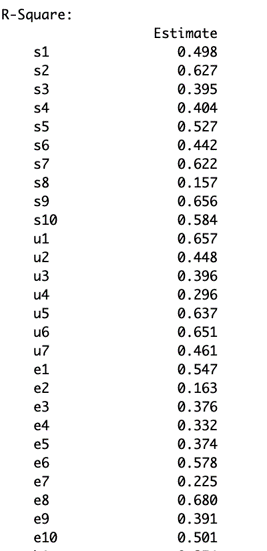
\includegraphics[t]{figures/cfatrimming.png}
%		\caption{Trimming the CFA Model.}
%		\label{fig:cfatrimming}
%	\end{subfigure}
%\end{figure*}

%\begin{figure*}
%	\centering
%	\begin{subfigure}{.7\textwidth}
%		\centering
%		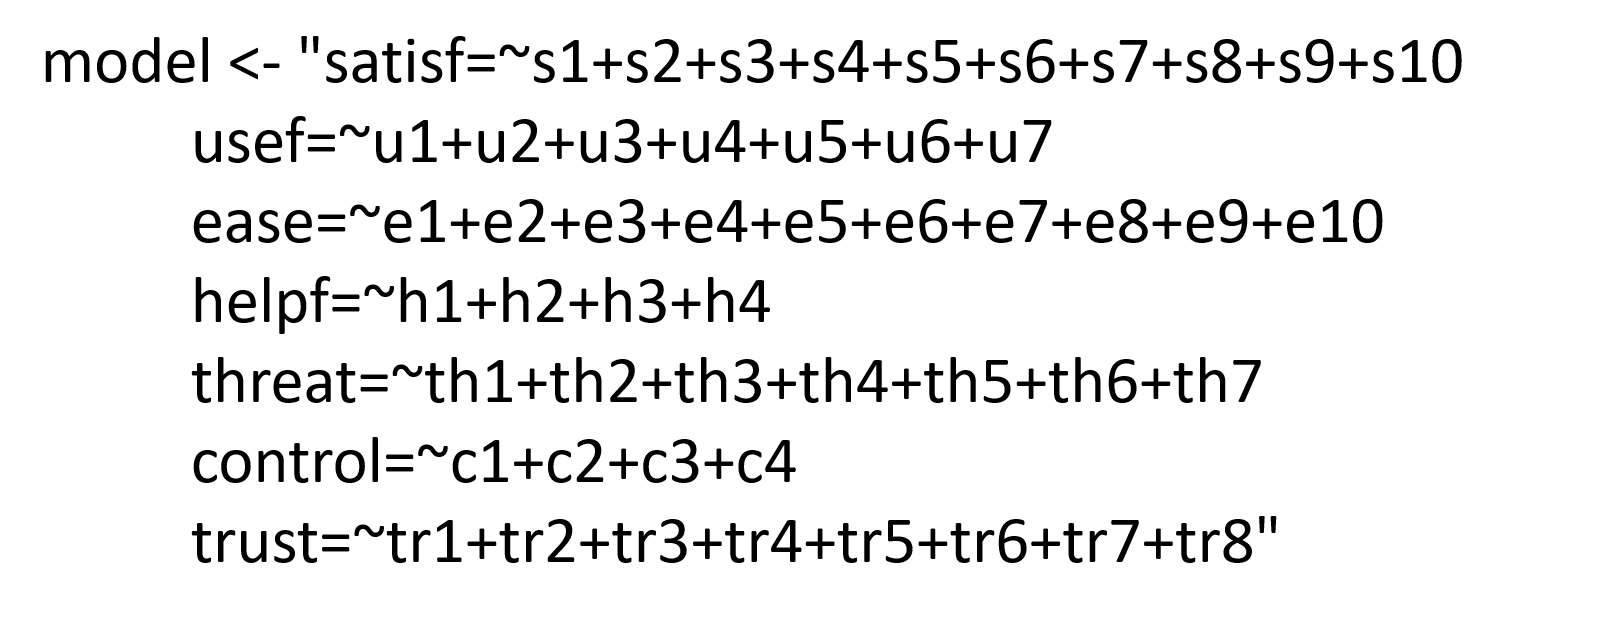
\includegraphics[width=\textwidth]{figures/cfasaturated.png}
%		\caption{CFA Saturated Model.}
%		\label{fig:cfasaturated}
%	\end{subfigure}%
%	\begin{subfigure}{.3\textwidth}
%		\centering
%		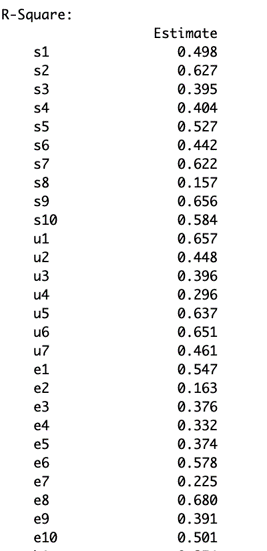
\includegraphics[width=\textwidth]{figures/cfatrimming.png}
%		\caption{Trimming the CFA Model by removing item with the lowest r-square}
%		\label{fig:cfatrimming}
%	\end{subfigure}
%	\caption{CFA Process}
%	\label{fig:test}
%\end{figure*}

\begin{figure}
	\centering
	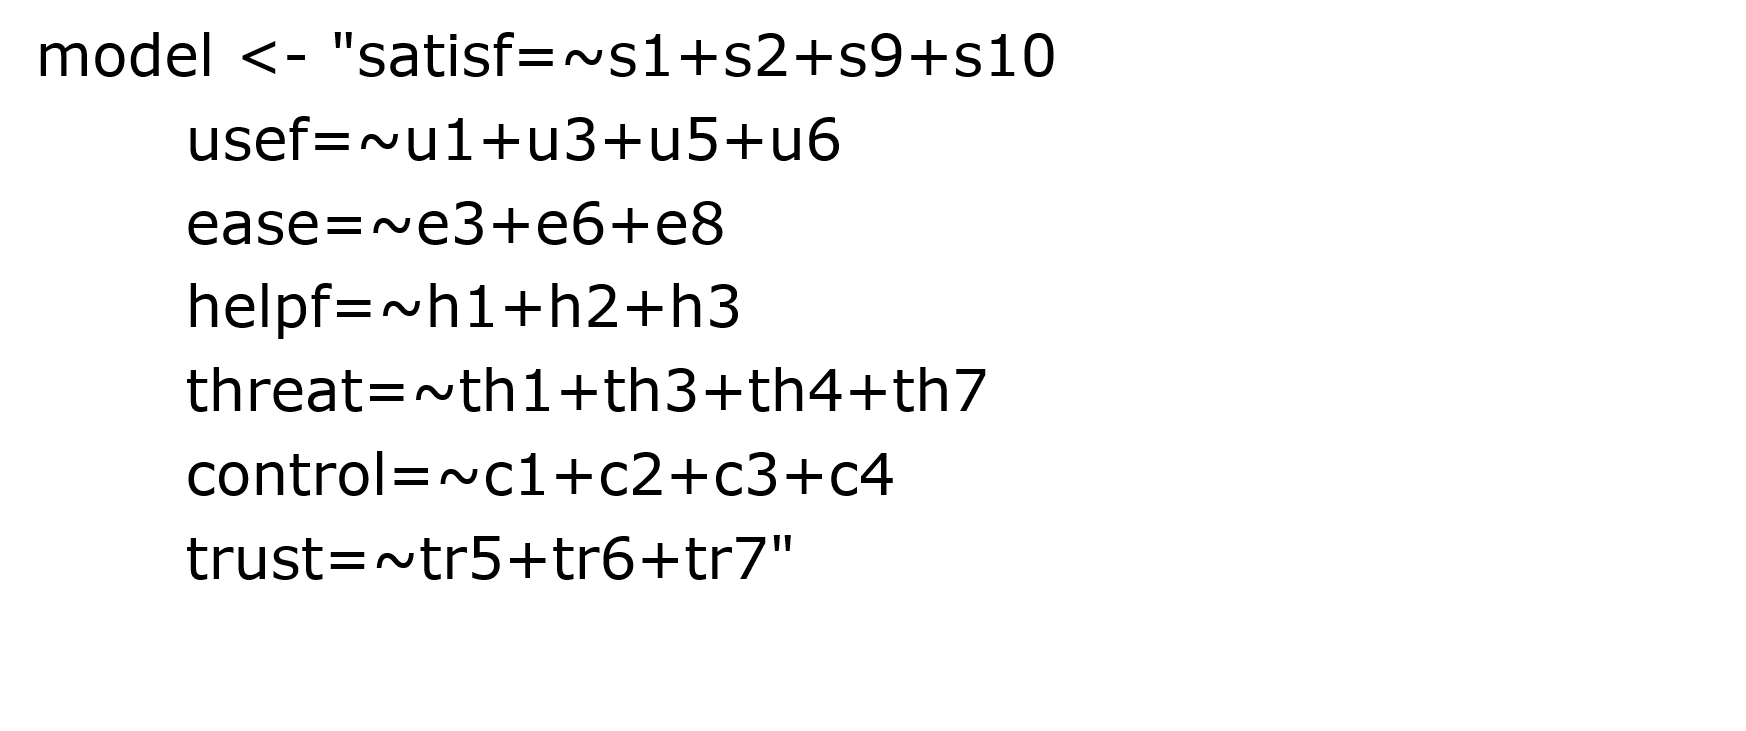
\includegraphics[width=0.7\textwidth]{figures/cfafinalmodel.png}
	\caption{Trimmed CFA Model.}
	\label{fig:cfafinalmodel}
\end{figure}

%\begin{figure}
%	\centering
%	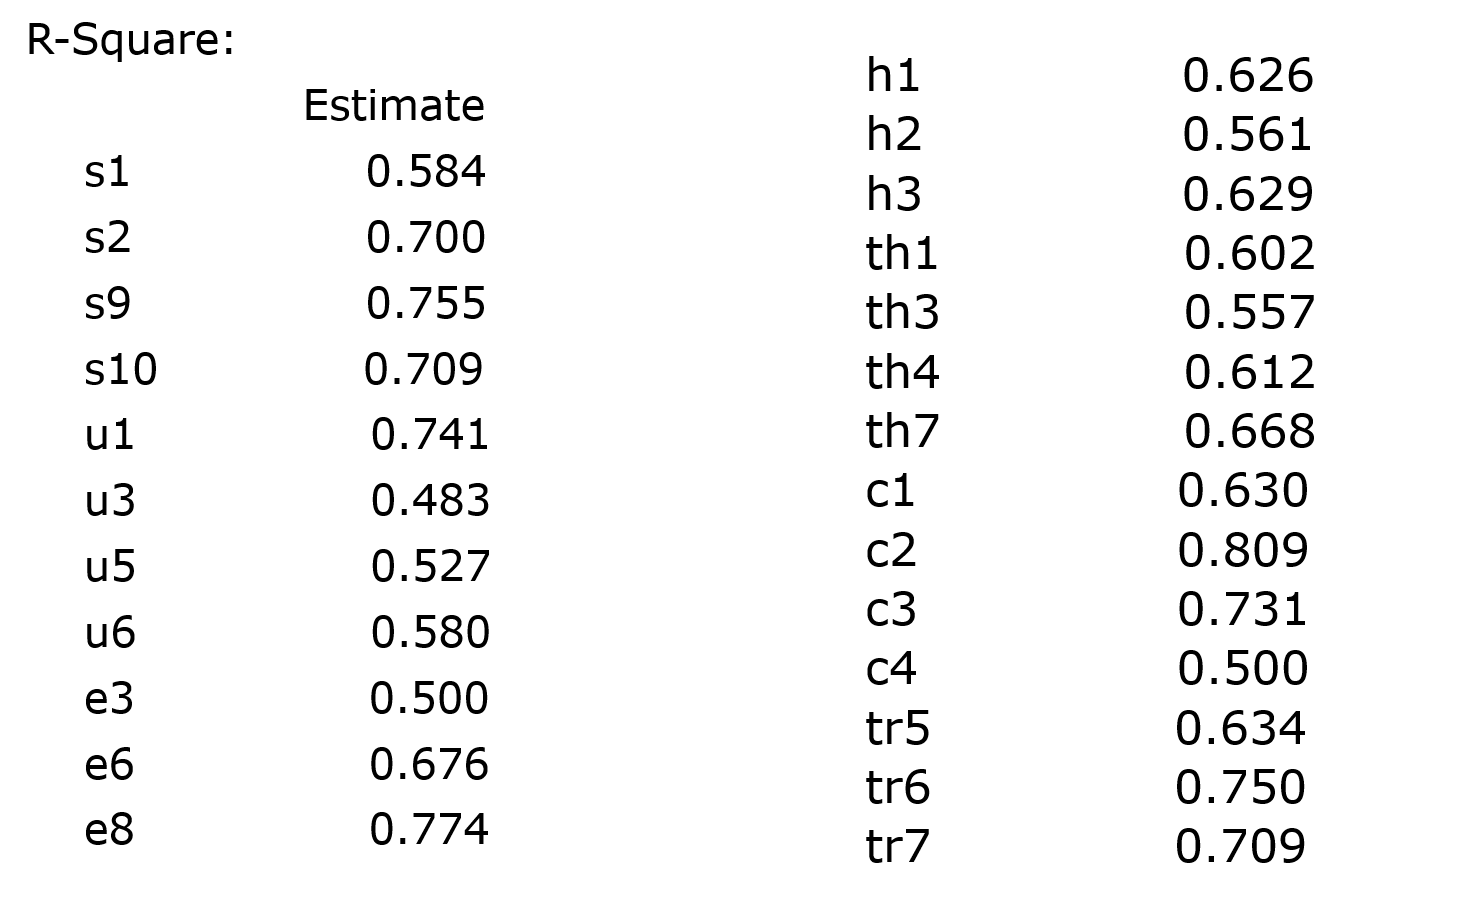
\includegraphics[width=0.5\textwidth]{figures/finalrsquare.png}
%	\caption{R-square value of trimmed CFA Model.}
%	\label{fig:finalrsquare}
%\end{figure}

% Please add the following required packages to your document preamble:
% \usepackage[normalem]{ulem}
% \useunder{\uline}{\ul}{}
\begin{table}
	\scriptsize
	\centering
	\begin{threeparttable}
	\caption {Factor Items in Trimmed CFA Model\tnote{1}}\label{tab:cfa}
	\begin{tabular}{l|l|l}
		\hline
		Construct                                                                            & Item                                                                                                                                                                                                                                                                                                                                                                                                                                                                                                                                                                                                                                                                                                                                                                          & Loading                                                                                                                                           \\ \hline
		\begin{tabular}[c]{@{}l@{}}System\\ satisfaction\\ \\ \cite{hui2006online, xu2009role, xu2011personalization} \end{tabular}        & \begin{tabular}[c]{@{}l@{}}The system has no real benefit to me.\\ Using the system is annoying.\\ \textcolor{gray}{Using the system is a pleasant experience.} \\ \textcolor{gray}{Using the system makes me happy.} \\ \textcolor{gray}{Overall, I am satisfied with the system.} \\ \textcolor{gray}{I would recommend the system to others.} \\ \textcolor{gray}{I would use this system if it were available.} \\ \textcolor{gray}{I would pay a monthly fee to use this system.} \\ I would quickly abandon using this system.\\ It would take a lot of convincing for me to use this system. \end{tabular}                                                                                                                                                                                                                                                                                & \begin{tabular}[c]{@{}l@{}}0.584\\ 0.700\\ \\ \\ \\ \\ \\ \\ 0.755\\ 0.709\end{tabular}                                                           \\ \hline
		\begin{tabular}[c]{@{}l@{}}Trust\\ \\ \\ \cite{jarvenpaa1999consumer,metzger2004privacy} \end{tabular}                     & \begin{tabular}[c]{@{}l@{}}\textcolor{gray}{I believe the company providing this software is trustworthy in handling my information.} \\ \textcolor{gray}{I believe this company tells the truth and fulfills promises related to the information I provide.} \\ \textcolor{gray}{I believe this company is predictable and consistent regarding the usage of my information.} \\ \textcolor{gray}{I believe this company is honest when it comes to using the information I provide.} \\ I think it is risky to give my information to this company.\\ There is too much uncertainty associated with giving my information to this company.\\ Providing this company my information would involve many unexpected problems.\\ \textcolor{gray}{I feel safe giving my information to this company.} \end{tabular}                       & \begin{tabular}[c]{@{}l@{}} \\ \\ \\ \\ 0.634\\ 0.750\\ 0.709 \\ \\\end{tabular}                                                                               \\ \hline
		\begin{tabular}[c]{@{}l@{}}Perceived \\ Usefulness\\ \\ \\ \cite{davis1989perceived} \end{tabular}   & \begin{tabular}[c]{@{}l@{}}Based on what I have seen, the system is useful.\\ \textcolor{gray}{The system helps me more effectively set my privacy preferences.} \\ The system gives me more control over my Smart home devices.\\ \textcolor{gray}{The privacy setting task would be easier to finish with the help of this system.} \\ The system saves me time when I use it.\\ The system meets my needs.\\ \textcolor{gray}{The system does everything that I expect it to do.} \end{tabular}                                                                                                                                                                                                                                                                                                                                     & \begin{tabular}[c]{@{}l@{}} 0.741\\ \\ 0.483\\ \\ 0.527\\ 0.580\\ \\ \end{tabular} \\ \hline
		\begin{tabular}[c]{@{}l@{}}Perceived \\ Ease of Use\\ \\ \cite{davis1989perceived,knijnenburg2014increasing} \end{tabular}     & \begin{tabular}[c]{@{}l@{}}\textcolor{gray}{It is convenient to set my preferences in the system.} \\ \textcolor{gray}{It requires the fewest mouse-clicks possible to set my privacy preferences with the system.} \\ It takes too many mouse-clicks to set my privacy preferences with the system.\\ \textcolor{gray}{I was able to quickly set my privacy-setting preferences in the system.} \\ \textcolor{gray}{I feel setting my privacy preferences within the system is easy.} \\ I feel setting my preferences in the system was unnecessarily complex.\\ \textcolor{gray}{I can set my privacy-setting preferences without written instructions.} \\ I felt lost using the system’s privacy settings.\\ \textcolor{gray}{I felt this privacy-setting interface is designed for all levels of users.} \\ \textcolor{gray}{I can use the Privacy-setting interface successfully every time.} \end{tabular} & \begin{tabular}[c]{@{}l@{}} \\ \\ 0.500\\ \\ \\ 0.676\\ \\ 0.774 \\ \\ \\ \end{tabular}                            \\ \hline
		\begin{tabular}[c]{@{}l@{}}Perceived\\ privacy \\ Helpfulness\\ \cite{wang2007recommendation} \end{tabular}    & \begin{tabular}[c]{@{}l@{}}The system helped me to decide what information I should disclose.\\ The system explained how useful providing each piece of information was.\\ The system helped me to make a tradeoff between privacy and usefulness.\\ \textcolor{gray}{I felt clueless about what information to disclose.} \end{tabular}                                                                                                                                                                                                                                                                                                                                                                                                                                                         & \begin{tabular}[c]{@{}l@{}}  0.626\\ 0.561\\ 0.629\\ \\ \end{tabular}                            \\ \hline
		\begin{tabular}[c]{@{}l@{}}Perceived\\ Privacy\\ Threat\\ \\ \cite{knijnenburg2014increasing} \\ \end{tabular} & \begin{tabular}[c]{@{}l@{}}I am afraid that I am sharing my personal information too freely, due to my privacy settings.\\ \textcolor{gray}{I am comfortable with amount of data that is used/shared based on my settings.}\\ Due to the system, the manufacturer will know too much about me.\\ Due to the system, third-parties will know too much about me.\\ \textcolor{gray}{I made sure only information that I am comfortable with will be used or shared.} \\ \textcolor{gray}{My privacy settings are spot on; I am not disclosing too much to anyone.}\\ I fear that I have been too liberal in selecting my privacy settings.\end{tabular}                                                                                                                                                            & \begin{tabular}[c]{@{}l@{}} 0.602\\ \\ 0.557\\ 0.612\\ \\ \\ 0.668\end{tabular} \\ \hline
		\begin{tabular}[c]{@{}l@{}}Perceived\\ Control\\ \cite{xu2012research} \\ \end{tabular}          & \begin{tabular}[c]{@{}l@{}}I had limited control over the way this system made privacy settings.\\ The system restricted me in my choice of settings.\\ Compared to how I normally configure privacy settings, the system was very limited.\\ I would like to have more control over the recommendations.\end{tabular}                                                                                                                                                                                                                                                                                                                                                                                                                                                        & \begin{tabular}[c]{@{}l@{}}0.630\\ 0.809\\  0.731\\ 0.500\end{tabular} \\ \hline
	\end{tabular}
	\begin{tablenotes}
		\item[1] Grayed out items were removed during trimming
	\end{tablenotes}
	\end{threeparttable}
\end{table}

Also, to ensure the convergent validity of constructs, I examined the average variance extracted (AVE) of each construct. The AVEs were all higher than the recommended value of 0.50, indicating adequate convergent validity. To ensure discriminant validity, we ascertained that the square root of the AVE for each construct was higher than the correlations of the construct with other constructs. As shown in Figure~\ref{fig:FactorCorrelationMatrix}\footnote{on the diagonal is the sqrt(AVE)}, trust, satisfaction, perceived privacy threat, perceived ease of use, and perceived control all have high correlation with each other (at least 0.746). Out of them, perceived privacy threat and perceived ease of use have the lowest AVE but with the highest correlation with other constructs. And if these two constructs are removed from the model, the square root of the AVE for other construct will be higher than their correlations with the left constructs, which indicates the discriminant validity. Thus, we removed perceived privacy threat and perceive ease of use from the final model.
The model has a following model fit: ${\chi}^{2}(125) = 298.507, p = .0000; RMSEA =
0.067, 90\% CI: [0.058, 0.077], CFI = 0.975, TLI = 0.970$.
%\begin{table}[]
%	\begin{tabular}{l|l|l|l|l|l|l|l|l}
%		\hline
%		& AVE   & Satisfaction & Usefulness & Trust  & Ease   & Helfpf & Threat & Control \\ \hline
%		Satisfaction & 0.829 & 0.829        & -0.383     & 0.486  & 0.440  & -0.003       & 0.442  & 0.476   \\ \hline
%		Usefulness   & 0.763 & -0.383       & 0.763      & -0.268 & -0.225 & 0.416        & -0.202 & -0.172  \\ \hline
%		Trust        & 0.835 & 0.486        & -0.268     & 0.835  & 0.467  & 0.027        & 0.543  & 0.507   \\ \hline
%		Ease of use  & 0.806 & 0.440        & -0.225     & 0.467  & 0.806  & 0.044        & 0.466  & 0.477   \\ \hline
%		Helfulness   & 0.778 & -0.003       & 0.416      & -0.027 & 0.044  & 0.778        & 0.035  & 0.126   \\ \hline
%		Threat       & 0.780 & 0.442        & -0.202     & 0.543  & 0.466  & 0.035        & 0.780  & 0.507   \\ \hline
%		Control      & 0.817 & 0.476        & -0.172     & 0.507  & 0.477  & 0.126        & 0.507  & 0.817   \\ \hline
%	\end{tabular}
%	\caption {Factor Correlation Matrix}\label{tab:CorrelationMatrix}
%\end{table}

\begin{figure}
	\centering
	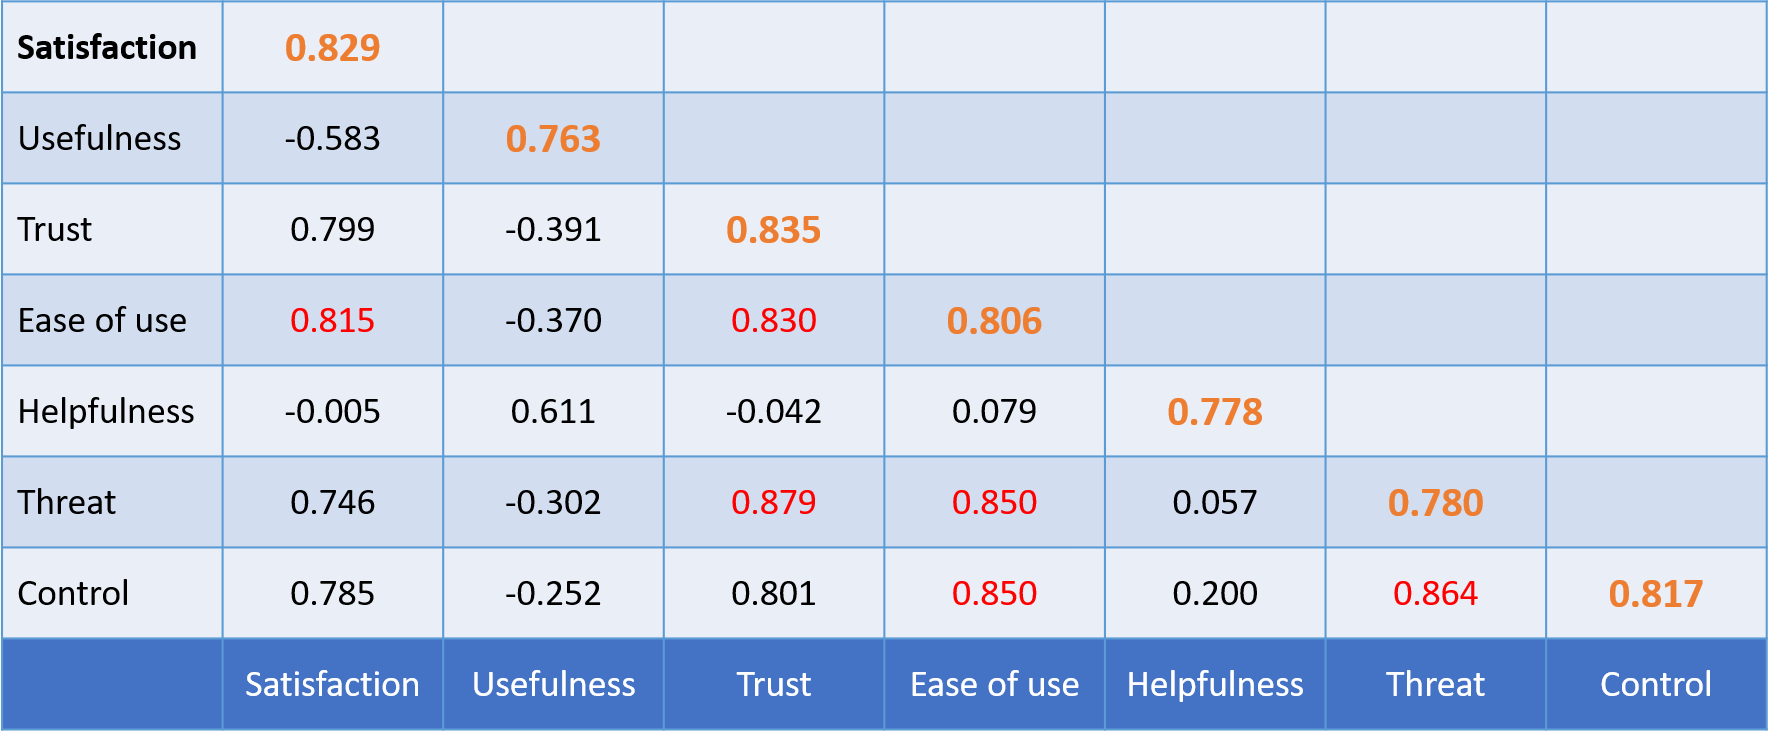
\includegraphics[width=\textwidth]{figures/FactorCorrelationMatrix.png}
	\caption{Factor Correlation Matrix (on the diagonal is the sqrt(AVE)).}
	\label{fig:FactorCorrelationMatrix}
\end{figure}

\subsection{Structural Equation Modeling}

I tried many different SEM models. Figure~\ref{fig:semmodel1} shows a model which contains perceived privacy threat, perceived helpfulness, and perceived usefulness. This model has a good model fit. However, the user experience variables --- satisfaction and trust are both removed from the model due to the high covariance between them and perceived privacy threat. Thus, this model was not chosen.
\begin{figure}
	\centering
	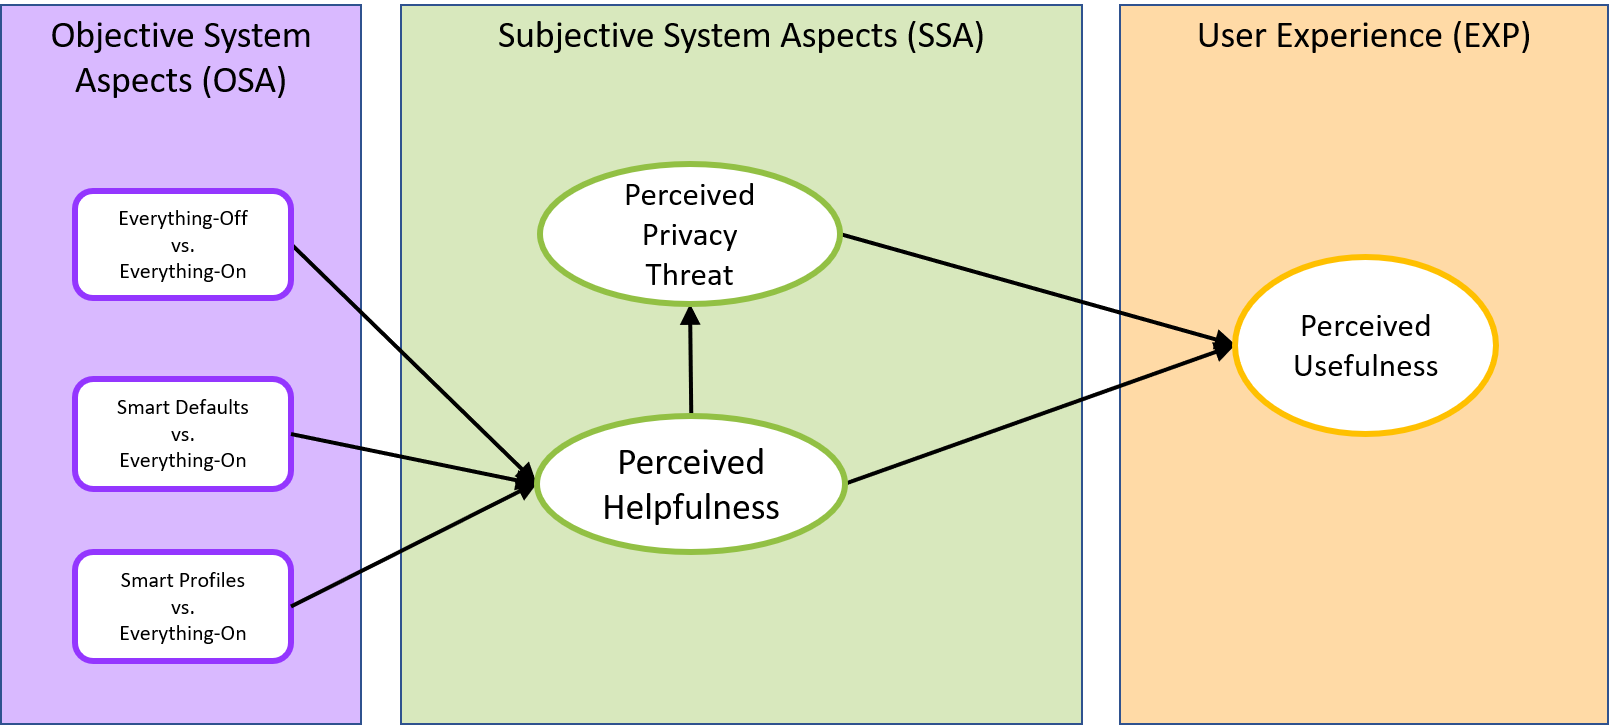
\includegraphics[width=0.85\textwidth]{figures/semmodel1.png}
	\caption{Preliminary SEM Model with perceived privacy threats}
	\label{fig:semmodel1}
\end{figure}

As shown in Figure~\ref{fig:semmodel2}, I also tried another model with hypothesizing that there will be significant effect from objective system aspects (experimental conditions/manipulations) to perceived control since. Compared to the previous preliminary model, this model kept satisfaction and perceived usefulness. Both of these factors are mediated by the perceived control and perceived helpfulness. However, no significant effect from the manipulations to the perceived control was found.
\begin{figure}
	\centering
	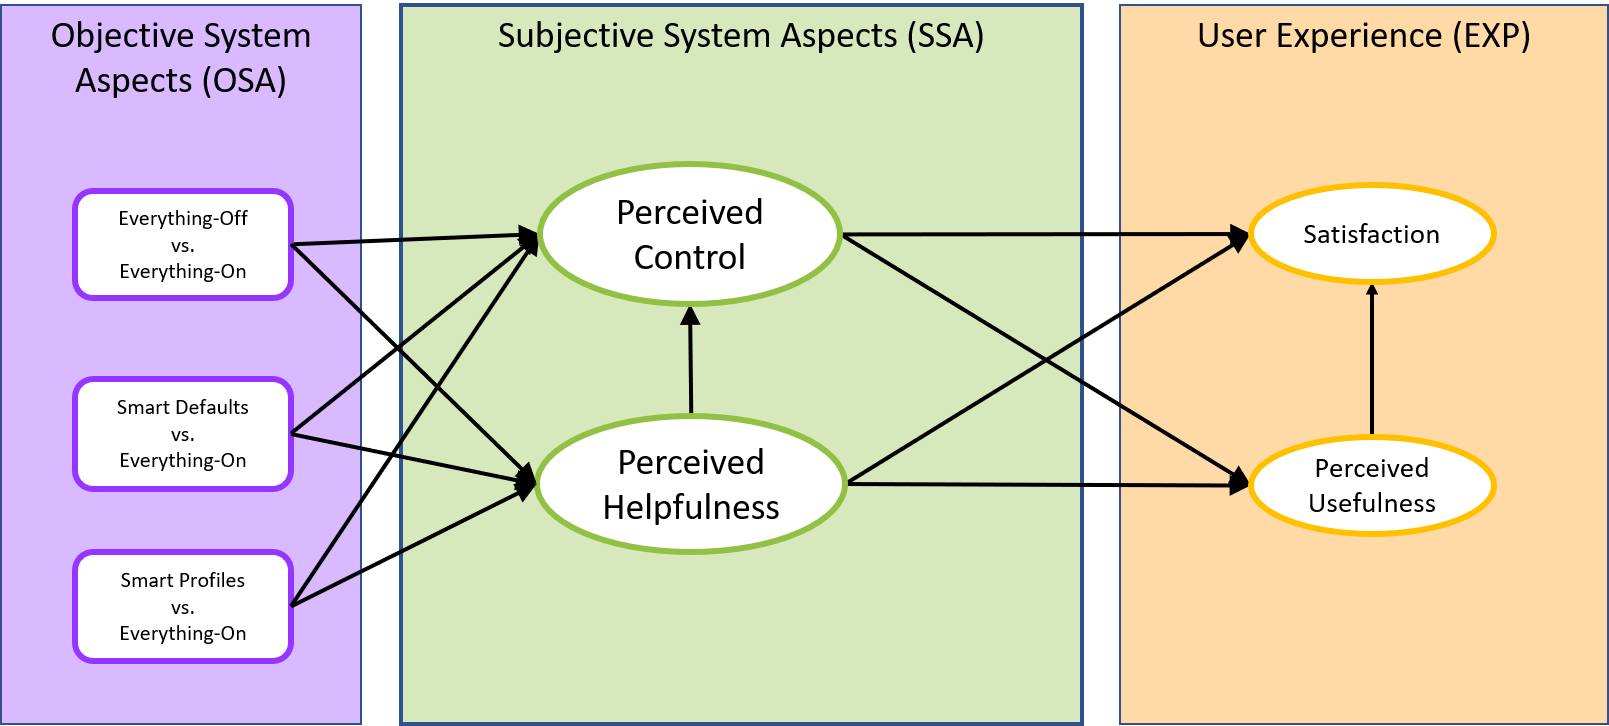
\includegraphics[width=0.85\textwidth]{figures/semmodel2.png}
	\caption{Preliminary SEM Model with effect from manipulations to perceived control}
	\label{fig:semmodel2}
\end{figure}

Finally, as shown in Figure~\ref{fig:finalcoremodel}, we subjected the remaining 5 factors (Trust, Satisfaction, Perceived Usefulness, Perceived Control, and Perceived Helpfulness) and the experimental conditions to structural equation modeling, which simultaneously fits the factor measurement model and the structural relations between factors and other variables. The model has following model fit: ${\chi}^{2}(176) = 284.160, p = .0000; RMSEA = 0.045, 90\% CI: [0.035, 0.054], CFI = 0.986, TLI = 0.983$.

\begin{figure}
	\centering
	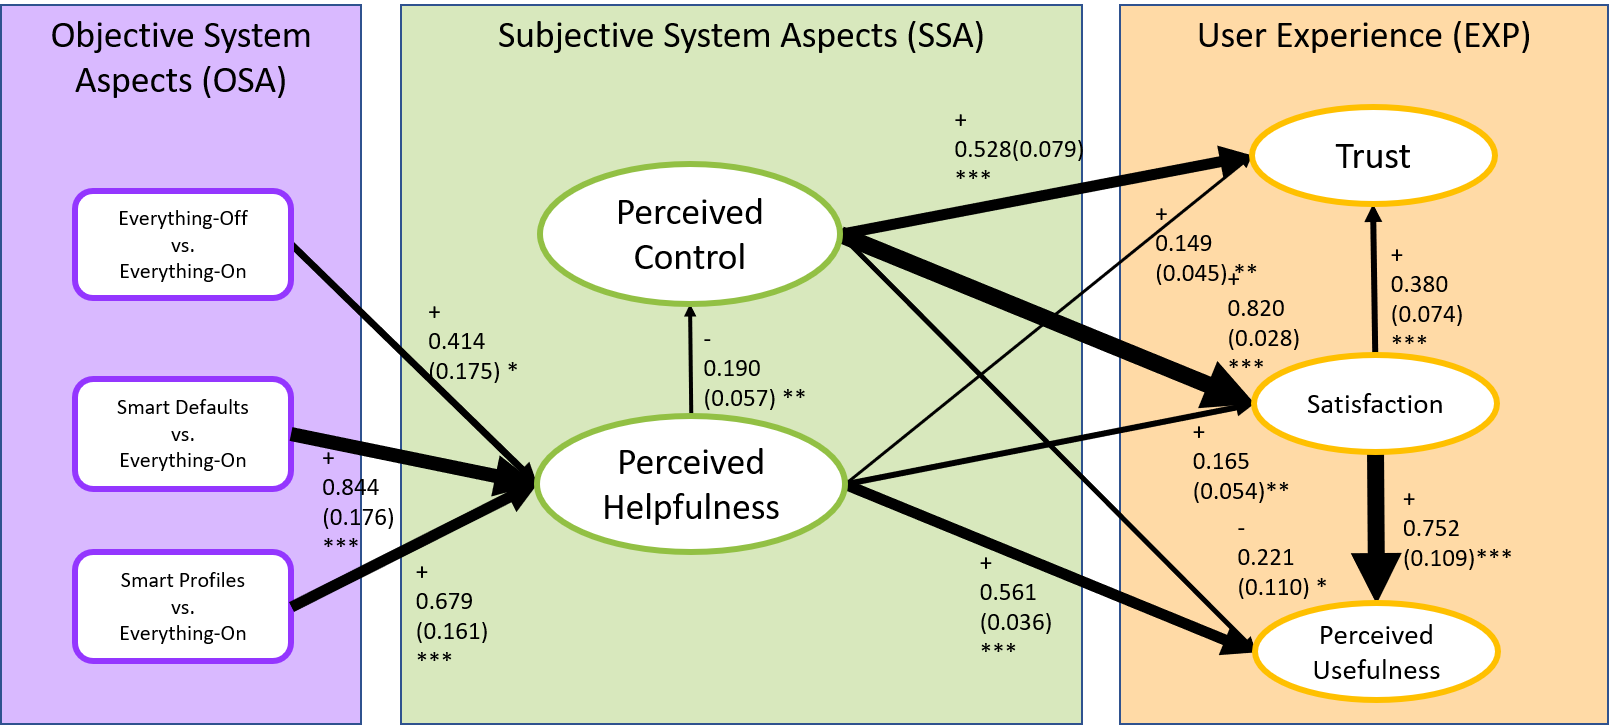
\includegraphics[width=0.85\textwidth]{figures/sem_model.png}
	\caption{ Trimmed structural equation model. $* p < .05, ** p < .01, *** p < .001$.}
	\label{fig:finalcoremodel}
\end{figure}

The model answers the two first two research questions --- smart defaults/profiles manipulation has a significant effect on the helpfulness of the system: Participants in Everything-Off, Smart Defaults, and Smart Profiles conditions perceived more helpfulness than the Everything-On condition. The two different UIs, however, do not have a significant effect on anything.

\begin{figure}
	\centering
	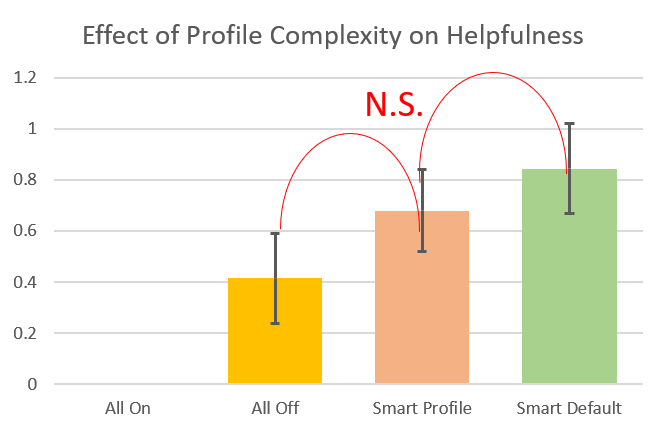
\includegraphics[width=0.5\textwidth]{figures/effectonhelpfulness.png}
	\caption{Effects of profile complexity on perceived helpfulness}
	\label{fig:effectonhelpfulness}
\end{figure}

Figure~\ref{fig:effectonhelpfulness} shows the effect of profile complexity on perceived helpfulness. Both Everything-On and Everything-Off have been used as the baseline to test the significance of the effect. The results shows that only the difference between pair (Everything-off -- smart profiles) and pair (smart profiles --- smart defaults) are not significant. The effect between all other manipulations are significant.

The helpfulness is in turn related to users' perceived control. Here we see that perceived helpfulness has a negative effect on users' perceived control. This indicates an interesting debate between perceived control and perceived helpfulness from the users. More details about this debate will be discussed in the next section. Figure~\ref{fig:effectoncontrol} shows the total effects of profile complexity on perceived control. All the effects are significant, which indicates that the effect of profile complexity on perceived control is mediated by perceived helpfulness. 

\begin{figure}[ht]
	\centering
	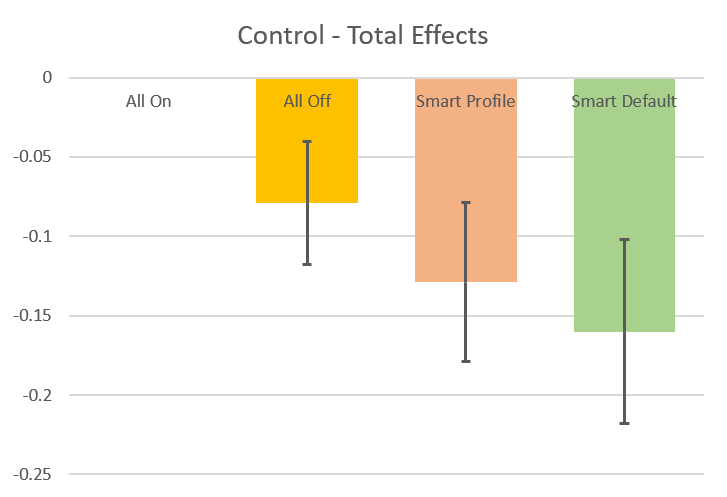
\includegraphics[width=0.5\textwidth]{figures/effectoncontrol.png}
	\caption{Total Effects of profile complexity on perceived control}
	\label{fig:effectoncontrol}
\end{figure}

%Control in turn has a significant positive effect on satisfaction and trust.
Both the perceived control and perceived helpfulness have a positive significant effect on users' satisfaction with the system. Figure~\ref{fig:effectoncontrol} shows the total effects of profile complexity on satisfaction. No significant effect was found. This, in the other hand, also proofs that the debating between perceived control and perceived helpfulness are canceling the effect from the manipulations on satisfaction.

\begin{figure}[ht]
	\centering
	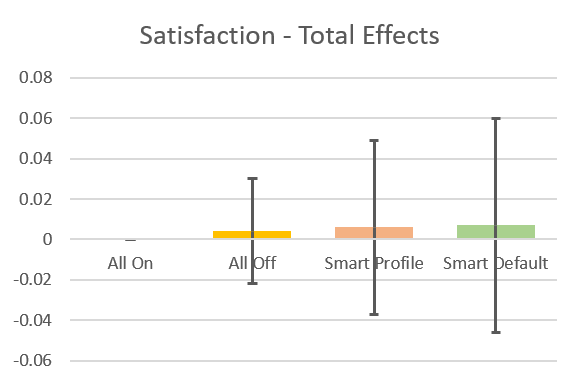
\includegraphics[width=0.5\textwidth]{figures/effectonsatisfaction.png}
	\caption{Total Effects of profile complexity on satisfaction}
	\label{fig:effectonsatisfaction}
\end{figure}

Perceived control, Perceived helpfulness, and the satisfaction all have significant positive effects on users' trust in the company. Figure~\ref{fig:effectoncontrol} shows the total effects of profile complexity on trust. No significant effect was found. Thus, the effect from the manipulations on trust were also being canceled by the debating between perceived control and perceived helpfulness.

\begin{figure}[ht]
	\centering
	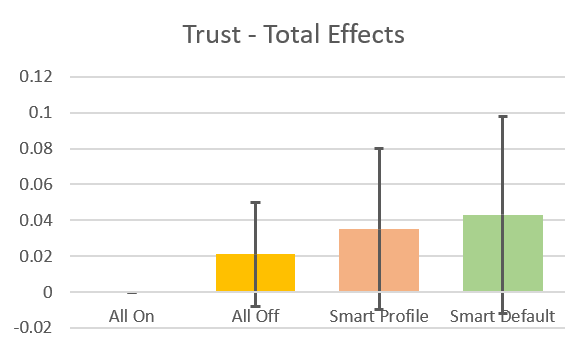
\includegraphics[width=0.5\textwidth]{figures/effectontrust.png}
	\caption{Total Effects of profile complexity on trust}
	\label{fig:effectontrust}
\end{figure}

Perceived control, Perceived helpfulness, and the satisfaction all determine perceived usefulness. Both satisfaction and perceived helpfulness have a positive significant effect on perceived usefulness. Perceived control has a negative significant effect on perceived usefulness. Less perceived control indicates there were more perceived helpfulness. And more perceived helpfulness could lead to more perceived usefulness. Figure~\ref{fig:effectoncontrol} shows the total effects of profile complexity on perceived usefulness. All the effects are significant. This may be due to the effect from perceived helpfulness on perceived usefulness is strong and the effect from perceived control is weak. Also, the covariance between perceived helpfulness and perceived usefulness is 

\begin{figure}
	\centering
	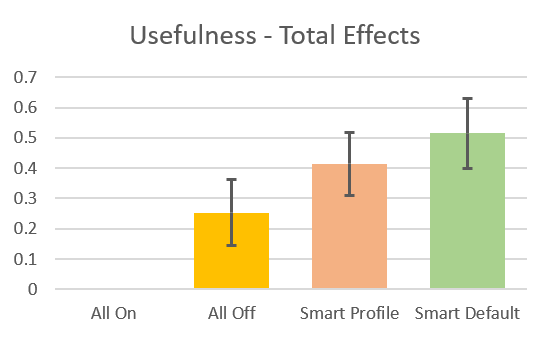
\includegraphics[width=0.5\textwidth]{figures/effectonusefulness.png}
	\caption{Total Effects of profile complexity on usefulness}
	\label{fig:effectonusefulness}
\end{figure}



%We also investigated the total effect of experimental conditions on the user experience and subjective system aspects. The results show that the manipulation of the complexity of profile only have significant total effect on perceived control and perceived userfulness, as shown in Table~\ref{tab:totaleffect}.

%\begin{table}
%	\begin{tabular}{l|l|l|l}
%		\hline
%		& Estimate & S.E.  & p-Value \\ \hline
%		Effects from Everything-Off to control    & 0.079    & 0.039 & 0.044   \\\hline
%		Effects from Smart Defaults to control    & 0.160    & 0.058 & 0.005   \\\hline
%		Effects from Smart Profiles to control    & 0.129    & 0.050 & 0.010   \\\hline
%		Effects from Everything-Off to usefulness & 0.252    & 0.109 & 0.020   \\\hline
%		Effects from Smart Defaults to usefulness & 0.515    & 0.115 & 0.000   \\\hline
%		Effects from Smart Profiles to usefulness & 0.414    & 0.105 & 0.000  \\\hline
%	\end{tabular}
%	\caption{Total Effect from experimental conditions on control and usefulness}\label{tab:totaleffect}
%\end{table}

\section{Discussion}
In this chapter we conducted a systematic evaluation of the effect of several design parameters of a household IoT privacy settings interface on users’ evaluation of the system. In terms of managerial implications, we find that it is useful to utilize the data-driven approach to develop ``smart defaults" and ``smart profiles", and corresponding setting interfaces to improve users' experience and satisfaction. We did not find significant difference between the two UIs. This could be explained that the difference between those two UIs are subtle and both of them are effective when integrating the smart defaults/profiles to them.

Regarding the negative effect from perceived helpfulness on perceived control, there are a few possible explanations: i) It is possible that participants in ``smart defaults" and ``smart profiles" condition found their privacy-settings have already been set by defaults. Thus, they found those ``smart defaults" and ``smart profiles" generated from previous study are helpful. However, in the other hand, users may feel that their choice of settings have been limited due to these helpful pre-settings. ii) It is also possible that users feel as though the pre-set settings are helpful but also complicated. They feel they do not have control over these settings. These are also corresponding to our previous discussion on the trade-off between accuracy and parsimony. A more parsimonious profile would be easier to explain to the users and also make them less worried about the pre-defined settings. So users are debating between the benefit brought by the ``smart defaults" and ``smart profiles" and the control they like to have over these privacy settings of their household IoT devices.
iii) We also revisit the perceived scale that we used. It appear that all the items in that scale are reversed framed and related to the spirit of ``losing control" and having limited control when using the system. One example is question C4, ``I would like to have more control over the recommendations". Our system is all about make privacy setting recommendations. While we are making the right recommendation about the IoT privacy settings for users, they might still want more control and configure these settings by themselves, leading less control perceived.

Another interest point is that the lack of difference between smart default and smart profiles. We first investigated the time spent on the two conditions. Figure~\ref{fig:timeonui} shows the effect size of average time spent on different UI pages. Although the average time spent on smart defaults is higher than the smart profiles condition, the effect is not significant. So this could not be explained by the lack of interaction due to less time spent on the smart profiles than the smart defaults.

\begin{figure}
	\centering
	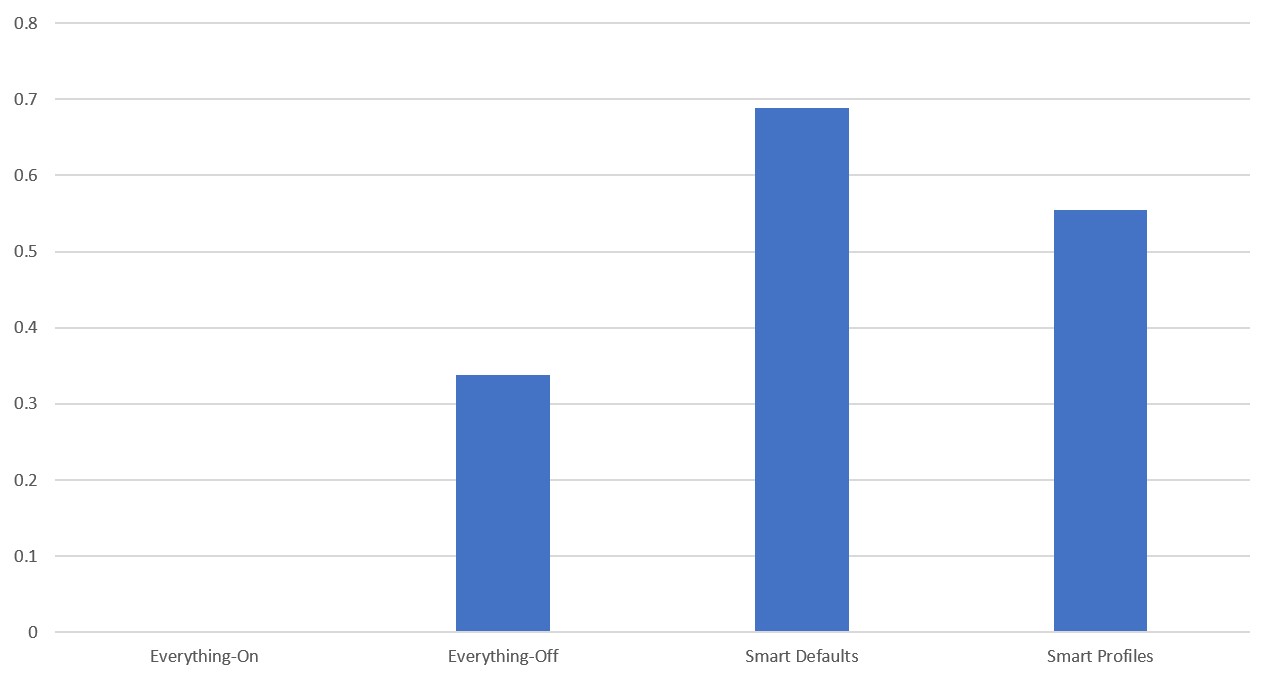
\includegraphics[width=0.8\textwidth]{figures/timeonui.png}
	\caption{Effect size of average time spent on different UI pages}
	\label{fig:timeonui}
\end{figure}

The finding is still interesting since users are expected to spend less time on smart profiles. And these lack of difference between smart defaults and smart profiles could be due to following reasons:

i) \textbf{Laziness?} Since in our smart profiles conditions for both interfaces, there are detailed description about the profile being showed. Thus, users would know what the setting will be like for smart profile condition. However, for smart defaults condition, users would not know what settings have been set there without going through all the settings. Thus, this could lead more time spent on the smart defaults UI page and better user experience.

ii) \textbf{Accuracy?} The second possible reason could be that the accuracy of the smart profiles are better than the smart defauls that we used. The higher accuracy the pre-settings are, the more likely users would make less changes and leave the settings as is, leading less time spent on the smart profiles UI page.

ii) \textbf{Endowment effect?} Since the smart defaults are provided by the system, while in the smart profile condition, users have to choose their own profile by reading the description of the profile. They might think they have already made the effort by reading the description and making the decision on choosing their favorite profile. Thus, they might think the profile that they chose fits their preference the best and would not take a deeper look or give more careful review on the settings in that profile.

There are several limitations to our work. First of all, our sample is not large enough to carefully examine 2- or 3-way interaction effects in M-plus. We examined the effect of personal characteristics on the user experience individually, and did not find any significant effect. A larger sample is needed to test these effects and assure the robustness of our results. Second, we planned to examined the behavior data that how users make the changes to the pre-defined settings. However, due to the coding problem, we were not able to access data. This should be improved in the next user study since users' setting behavior could give us more hints to explain our previous findings.

From the results of this study, we encourage privacy researchers, policy-makers, and industry executives to consider the effects of privacy settings interfaces on privacy outcomes. This paper shows that subtle changes in the design of such interfaces can have important subjective and behavioral consequences. Careful design of these systems is help users better setting their IoT devices.
